\subsection{Lindner-Peikert \NPs Algorithm} \label{sec:LPNP}
\begin{figure}
	\begin{subfigure}[b]{0.32\textwidth}
	\centering
	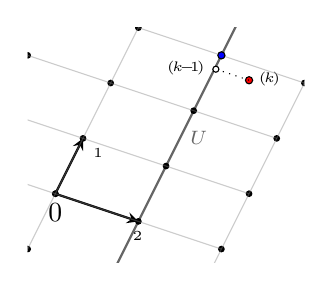
\begin{tikzpicture}
		\clip (-10pt,-25pt) rectangle (90pt, 60pt);
			%\draw[step=10pt,gray,opacity=0.1, very thin] (-40pt,-30pt) grid (100pt, 100pt);
			\foreach \y in {-2,...,5}
			\foreach \x in {-2,...,3}
			\filldraw(\x*40pt+\y*10pt, 10pt*\x+20pt*\y) circle (1pt);
			\filldraw(0pt,0pt) circle (1pt) node[below]{$0$};

			\draw[->, -stealth, black, thick] (0,0) -- (30pt, -10pt) node[font=\tiny, below]{$\bvec_2$};
			\draw[->, -stealth, black, thick] (0,0) -- (10pt, 20pt) node[font=\tiny, below right]{$\bvec_1$};
			\filldraw[fill=red](70pt, 41pt) circle (1.3pt) node[font=\tiny, right]{$\tvec^{(\mkern-2mu k \mkern-2mu)}$};
			%vertical lines:
			%\draw[gray, opacity=0.4] (-40pt, -10pt) -- (0pt, 70pt);
			\draw[gray, opacity=0.4] (-20pt, -40pt) -- (40pt, 80pt);
			\draw[black, thick, opacity=0.6] (20pt, -30pt) -- (70pt, 70pt) node[font=\scriptsize, midway, right]{$U$};
			\draw[gray, opacity=0.4] (50pt, -40pt) -- (90pt, 40pt);

			%horizontal lines:
			\draw[gray, opacity=0.4] (-30pt, 10pt) -- (60pt, -20pt);
			\draw[gray, opacity=0.4] (-20pt, 30pt) -- (70pt, 0pt);
			\draw[gray, opacity=0.4] (-40pt, 60pt) -- (80pt, 20pt);
			\draw[gray, opacity=0.4] (30pt, 60pt) -- (90pt, 40pt);
			%\draw[gray, opacity=0.4] (-50pt, -30pt) -- (70pt, 0pt);	
			
			%projection
			\draw[black, dotted] (70pt, 41pt) -- (58pt, 45pt);
			\filldraw[fill=white](58pt, 45pt) circle (1.1pt) node[font=\tiny, left] {$\tvec^{(\mkern-2mu k\mkern-3mu - \mkern-4mu 1 \mkern-2mu)}$};
			
			%solution
			\filldraw[fill=blue](60pt, 50pt) circle (1.3pt) node[font=\tiny, right]{$\vvec$};
	\end{tikzpicture}
	\caption{\scriptsize Babai's $\NP$ Algorithm on a `good' basis. The target point $t^{(k)}$ (red) is projected onto the closest hyperplane $U=\bvec_2+\Span(\bvec_1).$ The recursive call for this 1-dimensional $U$ projects $\tvec^{(k-1)}$ onto the closest zero-dimensional subspace, i.e.\ lattice point $\vvec$ (blue). }
                \label{fig:NP1}
	\end{subfigure}%
	~
    \begin{subfigure}[b]{0.32\textwidth}
    		\centering
    		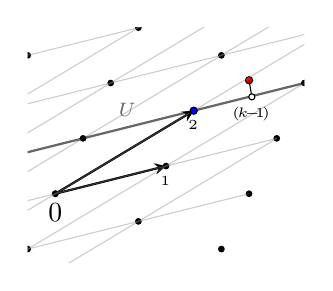
\begin{tikzpicture}
		\clip (-10pt,-25pt) rectangle (90pt, 60pt);
			\foreach \y in {-2,...,5}
			\foreach \x in {-2,...,3}
			\filldraw(\x*40pt+\y*10pt, 10pt*\x+20pt*\y) circle (1pt);
			\filldraw(0pt,0pt) circle (1pt) node[below]{ $0$};

			\draw[->, -stealth, black, thick] (0,0) -- (40pt, 10pt) node[font=\tiny, below]{$\bvec_1$};
			\draw[->, -stealth, black, thick] (0,0) -- (50pt, 30pt) node[font=\tiny, below]{$\bvec_2$};
			\filldraw[fill=red](70pt, 41pt) circle (1.3pt) node[font=\tiny, right]{$\tvec$};
			%vertical lines:
			\draw[gray, opacity=0.4] (-50pt, -30pt) -- (100pt, 60pt);
			\draw[gray, opacity=0.4] (-40pt, -10pt) -- (110pt, 80pt);
			\draw[gray, opacity=0.4] (-30pt, 10pt) -- (70pt, 70pt);
			\draw[gray, opacity=0.4] (-70pt, 0pt) -- (80pt, 90pt);
			\draw[gray, opacity=0.4] (-60pt, -50pt) -- (90pt, 40pt);
			\draw[gray, opacity=0.4] (-20pt, -40pt) -- (80pt, 20pt);
			
			%horizontal lines:
			\draw[gray, opacity=0.4] (-50pt, 40pt) -- (70pt, 70pt);
			\draw[gray, opacity=0.4] (-60pt, 20pt) -- (100pt, 60pt);
			\draw[black, thick, opacity=0.6] (-70pt, 0pt) -- (90pt, 40pt) node[font=\scriptsize, above, pos=0.6]{$U$};
			\draw[gray, opacity=0.4] (-40pt, -10pt) -- (80pt, 20pt);
			\draw[gray, opacity=0.4] (-50pt, -30pt) -- (70pt, 0pt);	
			
			%projection 
			\draw[black] (70pt, 41pt) -- (71pt, 35pt);
			\filldraw[fill=white](71pt, 35pt) circle (1.1pt) node[font=\tiny, below] {$\tvec^{(\mkern-2mu k\mkern-3mu - \mkern-4mu 1 \mkern-2mu)}$};
			
			%solution
			\filldraw[fill=blue](50pt, 30pt) circle (1.3pt) node[font=\tiny, left, above]{$\vvec$};
			
	\end{tikzpicture}
	\caption{\scriptsize Babai's $\NP$ Algorithm on a `bad' basis for the same lattice. Now the target point $\tvec^{(k)}$ (red) is projected onto the hyperplane $U=\bvec_2+\Span(\bvec_1)$ but for different $\bvec_2, \bvec_1$, so the hyperplane has changed. The returned vector $\vvec$  is not the closest vector.}
	\label{fig:NP2}
    \end{subfigure}%
    ~
    \begin{subfigure}[b]{0.32\textwidth}
    		\centering
    		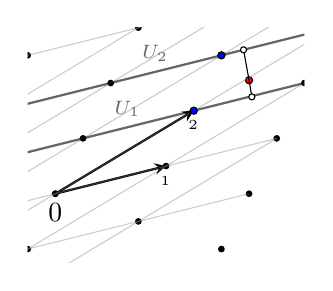
\begin{tikzpicture}
		\clip (-10pt,-25pt) rectangle (90pt, 60pt);
			%\draw[step=10pt,gray,opacity=0.1, very thin] (-40pt,-30pt) grid (100pt, 100pt);
			\foreach \y in {-2,...,5}
			\foreach \x in {-2,...,3}
			\filldraw(\x*40pt+\y*10pt, 10pt*\x+20pt*\y) circle (1pt);
			\filldraw(0pt,0pt) circle (1pt) node[below]{ $0$};

			\draw[->, black, -stealth, thick] (0,0) -- (40pt, 10pt) node[font=\tiny, below]{$\bvec_1$};
			\draw[->, black, -stealth, thick] (0,0) -- (50pt, 30pt) node[font=\tiny, below]{$\bvec_2$};
			\filldraw[fill=red](70pt, 41pt) circle (1.3pt) node[font=\tiny, right]{$\tvec$};
			%vertical lines:
			\draw[gray, opacity=0.4] (-50pt, -30pt) -- (100pt, 60pt);
			\draw[gray, opacity=0.4] (-40pt, -10pt) -- (110pt, 80pt);
			\draw[gray, opacity=0.4] (-30pt, 10pt) -- (70pt, 70pt);
			\draw[gray, opacity=0.4] (-70pt, 0pt) -- (80pt, 90pt);
			\draw[gray, opacity=0.4] (-60pt, -50pt) -- (90pt, 40pt);
			\draw[gray, opacity=0.4] (-20pt, -40pt) -- (80pt, 20pt);
			
			%horizontal lines:
			\draw[gray, opacity=0.4] (-50pt, 40pt) -- (70pt, 70pt);
			\draw[black, thick, opacity=0.6] (-60pt, 20pt) -- (100pt, 60pt) node[font=\scriptsize, above, pos=0.6]{$U_2$};
			\draw[black, thick, opacity=0.6] (-70pt, 0pt) -- (90pt, 40pt) node[font=\scriptsize, above, pos=0.6]{$U_1$};
			\draw[gray, opacity=0.4] (-40pt, -10pt) -- (80pt, 20pt);
			\draw[gray, opacity=0.4] (-50pt, -30pt) -- (70pt, 0pt);	
			
			%projections 
			\draw[black] (70pt, 41pt) -- (71pt, 35pt);
			\filldraw[fill=white](71pt, 35pt) circle (1.1pt);
			
			\draw[black] (70pt, 41pt) -- (68pt, 52pt);
			\filldraw[fill=white](68pt, 52pt) circle (1.1pt);
			
			%solutions
			\filldraw[fill=blue](50pt, 30pt) circle (1.3pt);
			\filldraw[fill=blue](60pt, 50pt) circle (1.3pt) node[font=\tiny, above]{$\vvec$};
	\end{tikzpicture}
	\caption{\scriptsize Lindner-Peikert $\NPs$ Algorithm on the same `bad' basis. We set $\dvec = (1, 2)$ and project the target $\tvec$ onto two hyperplanes $U_1 = \bvec_2+\Span(\bvec_1), U_2 = 2\bvec_2+\Span(\bvec_1)$. The output points are marked blue. The closets point $\vvec$ is found among them.}
	\label{fig:NP3}
    \end{subfigure}%
    \caption{$\NP$(\texttt{s}) Algorithms}
    \label{fig:NPAlgs}
\end{figure}

For Eq.~(\ref{eq:BabaiProof}) to be smaller than 0, which translates to a constant success probability for the Babai's \LWE decoding, the \BKZ parameter $\beta$ must be set almost as large as the lattice dimension $m$. For example, for parameters $q=\bigO(n^2), \alpha=\bigO(1/n^{3/2})$, Eq.~(\ref{eq:BabaiProof}) is smaller than 0 when $\beta > \frac{1}{2} \frac{m}{\ca - \tfrac{n}{m} \cq}$. Setting $m = 2 \frac{\cq}{\ca} n$ (as this choice minimizes $\beta$), yields $\beta > 2 \frac{\cq}{\ca^2}n \approx \frac{16}{9}n$. For such large $\beta$, the \BKZ reduction is not efficient. Choosing smaller $\beta$ and, hence, decreasing the running time of \BKZ reduction, leads to a super-exponentially small success probability of the decoding (case 1 in Thm.~\ref{thm:PsuccBabai}).

To amplify the success probability of Babai's algorithm (at the expense of its running time), Lindner and Peikert \cite{RSA:LinPei11} proposed an extended variant of the $\NP$ algorithm. Instead of choosing only one closest hyperplane $U_i$ (line \ref{algline:BabaiChoosePlane} in Alg.~\ref{alg:Babai}), we choose several, say $d$, close hyperplanes (line \ref{algline:LPChoosePlane} in Alg.~\ref{alg:LP}) and project the target vector onto them. This results in $d$ new targets which are, in turn, projected onto $d'$ several close hyperplanes (see Fig.~\ref{fig:NP3}). For example, Fig.~\ref{fig:TwoTreesLP} represents the case $m=3, \dvec = (3, 2, 1)$. Babai's $\NP$ algorithm corresponds to $\dvec = \vec{1}$.

Geometrically this idea amounts to stretching the search region $V_{\SubBabai} = \FP(\wBMat)$ to $V_{\SubLP} = \FP(\wBMat \cdot \DMat)$ for a diagonal matrix $\DMat$ having $(d_1, \ldots, d_m)$ on the main diagonal. In the end, we have $\prod_i d_i$ candidate error-vectors, out of which the shortest is chosen. 

The formal description of this algorithm, which we call the $\NPs$ algorithm, is given in Alg.~\ref{alg:LP}. In addition to a lattice and a target vector, the algorithm receives a vector $\dvec = (d_1, \ldots, d_m)$. Below we explain how to choose this vector.
%
% LP algorithm
%
\setlength{\intextsep}{\medskipamount}
\begin{algorithm}[h]
\caption{Lindner-Peikert $\NPs$ $(\BMat, \xvec, \protect \tvec, \dvec)$}
\label{alg:LP}
\textbf{Input:} $\BMat=(\bvec_1, \ldots, \bvec_m) \in \Z^{m \times m}, \xvec \in \Q^m, \tvec \in \xvec+\Span(\BMat), \evec' \in \Q^m$ \hfill \Comment $\evec'=\xvec=0$ in the initial call\\
\textbf{Output:} A set of pair $(\vvec, \evec')$ where $\vvec \in \Lat(\BMat)$ and $\evec' = \vvec - \tvec$
\begin{algorithmic}[1]
\State $\xvec^{(k)}\gets \xvec, \tvec^{(k)}\gets \tvec,\evec'^{(k)}\gets\evec'$. 
\State Let $\wBMat \gets \GSO(\BMat)$. 
\If {$k=0$} \Return $\{(\xvec,\evec') \}$
\EndIf
\State Compute $c^{(k)}_1 \gets \bigScProd{\tvec^{(k)}}{\frac{\wbvec_k}{\vphantom{\scalebox{1.6}x^2} \|\wbvec_k \|^2}}$
\State Compute $c^{(k)}_j = \bigScProd{\xvec^{(k)}}{\frac{\wbvec_k}{\vphantom{\scalebox{1.6}x^2} \|{\wbvec_k}\|^2}} + i^{(k)}_j$ for $i^{(k)}_j \in \Z, 1 \leq j \leq d_k$ s.t.\ $c^{(k)}_j$ are closest to $c^{(k)}_1$ \label{algline:LPChoosePlane}
	\For {\textbf{each} $(i^{(k)}_j, c^{(k)}_j)$} 
		\State $\xvec^{(k-1)}_j \gets \xvec^{(k)}+i^{(k)}_j \bvec_k$ \label{algline:LPChooseTranslate}
		\Comment $U_j^{(k-1)} = \xvec^{(k-1)}_j+\Lat(\BMat^{(k-1)})$ are the $d_k$ nearest planes
		\State $\evec'^{(k-1)}_j \gets \evec'^{(k)} + (c^{(k)}_1-c^{(k)}_j)\wbvec_k$ \label{algline:LPComputeError}
		\State $\tvec^{(k-1)}_j =\tvec^{(k)} - (c^{(k)}_1-c^{(k)}_j)\wbvec_k$ \label{algline:LPProjectTarget} \Comment Project onto $U_j^{(k-1)}$ 
\State \Return $\bigcup_j \NPs ((\bvec_1,\ldots,\bvec_{k-1}), \xvec^{(k-1)}_j,\tvec^{(k-1)}_j,\evec'^{(k-1)}_j, \dvec\mkern5mu)$
\EndFor
\end{algorithmic} 
\end{algorithm}

\paragraph{Analysis.} Like in the analysis of Babai's algorithm, we approximate the discrete Gaussian error $\evec$ sampled with parameter $\alpha q$ by a continuous one. Our goal is to determine a choice of $\dvec$ that guarantees a constant success probability and from such a choice, deduce the running time of the $\NPs$ algorithm. 

From \cite{RSA:LinPei11}, the success probability of the algorithm when applied to $m$ \LWE-samples is
\begin{equation} \label{eq:LPPSucc}
	\Psucc(\NPs) = \Pr[\evec \in \FP(\wBMat \DMat)] = \prod_{i=1}^{m} \Pr \Bigl[ | \ScProd{\evec}{\wbvec_i} | < \tfrac{d_i \| \wbvec_i \|^2}{2} \Bigr] = \prod_{i=1}^{m} \erf \Bigl( \tfrac{d_i \| \wbvec_i \|^2}{2 \alpha q} \Bigr),
\end{equation}
where $\erf = \frac{2}{\sqrt{\pi}} \int_0^x \exp(-t^2) \d t$. Tail-bounds on the Gaussian distribution (Eq.~(\ref{eq:TailBound})) suggest that if $\min_{1 \leq i \leq m} \frac{d_i \| \wbvec_i \|}{ \alpha q} = \smallo(1)$, then $\Psucc(\NPs) = \smallo(1)$. However, if $\min_{1 \leq i \leq m} \frac{d_i \| \wbvec_i \|}{ \alpha q} = \wLandau(\sqrt{\log m})$, then $\Psucc(\NPs) = 1 - \smallo(1)$.  Setting 
\begin{equation} \label{eq:dSeqLP}
	d_i = \Bigl\lceil \frac{\alpha q \cdot (\log m)^{c}}{ \| \wbvec_i \|} \Bigr\rceil
\end{equation}
for some constant $c > 1/2$, the decoding succeeds with probability almost 1. In case $\|\wbvec_1\| \gg \alpha q$ (which is the case for \LWE), we set the first $d_i$'s equal to $1$ and start increasing the sequence once $\| \wbvec_i \|$'s become equal or smaller than $\alpha q$. 

The recursive $\NPs$ Algorithm~\ref{alg:LP} has a tree-structure (see Fig.~\ref{fig:TwoTreesLP}) with the root corresponding to the initial call and every node is created by projecting the target onto one out of $d_i$ hyperplanes. As the result, each node on level $k$ has $d_{m-k+1}$ children. The superscripts for $\xvec^{(k)}, \evec'^{(k)}, \tvec^{(k)}$ denote the level, the root is on level $m$, the leaves are on level 0. Vectors $\xvec^{(k)}_j, \evec'^{(k)}_j, \tvec^{(k)}_j$ are the data associated to one node on level $k$, giving (1) a partial solution (w.r.t. the basis $\BMat$), (2) a partial error-vector (w.r.t. the basis $\wBMat$), and (3) a new target. 

Let $N_k$ be the number of nodes at level $k$ and $N$ be the total number of nodes. At the root we have $N_m = 1$. Down the tree, we have $N_k = \prod_{i=k+1}^m d_i$ and $N = \sum_{k=0}^m N_k$. The work done on a node is clearly polynomial in $m$, so the total complexity of Alg.~\ref{alg:LP} is $N \cdot \poly(m)$. The following theorem gives the value for $N$ when the $d_i$'s are set as in Eq.~(\ref{eq:dSeqLP}).

\begin{thm}[Analysis of the $\NPs$ Algorithm~\ref{alg:LP}] \label{thm:LPRunTime}
	Given a $\beta = \TLandau(n)$-\BKZ reduced basis that arises from $m = \TLandau(n)$ \LWE-samples with parameters $(n, q=\bigO(n^{\cq}), \alpha = \bigO(1 / n^{\ca}) )$ for positive constants $\cq >\ca$, the $\NPs$ Algorithm~\ref{alg:LP} with the $\dvec$ set as in Eq.~(\ref{eq:dSeqLP}), solves the Search-\LWE problem with success probability $1-\smallo(1)$ in time
	\begin{equation*}
T(\NP)=\poly(m) \cdot N = \begin{cases}
                  2^{\frac{1}{2} \bigl(\frac{m}{2\beta}-\ca + \frac{n}{m} \cq  \bigr)^2 (1+\smallo(1)) \cdot \beta\log\beta},			      \quad & \text{if }  \frac{m}{2 \beta} - \ca + \frac{n}{m} \cq  > 0  \\
                  \poly(m)                                     \quad&\text{if } \frac{m}{2 \beta} - \ca + \frac{n}{m}\cq  < 0,
                  \end{cases}
	\end{equation*}
and $\poly(m)$ memory (using depth-first search) assuming the Geometric Series Assumption holds and the \LWE error follows a continuous Gaussian distribution.
\end{thm}

\begin{proof}
	As in Thm.~\ref{thm:PsuccBabai}, under GSA, the inequality $\frac{m}{2 \beta} - \ca + \frac{n}{m}\cq  < 0$ translates into $\| \wbvec_m \| > \alpha q \cdot \poly(n)$. It immediately gives $d_i = \lceil \frac{\alpha q \cdot (\log m)^{c}}{ \alpha q \cdot \poly(n)} \rceil = 1$ (for some constant $c>1/2$ ). This is exactly Babai's $\NP$ algorithm which has $\poly(m)$ running time.
	
	In case $\frac{m}{2 \beta} - \ca + \frac{n}{m}\cq  > 0$, we have to increase some $d_i$'s to guarantee the desired success probability. Again as in Thm.~\ref{thm:PsuccBabai}, there exist a critical level $k^*$ s.t.\ $\| \wbvec_{k^*}\| > \alpha q$ and $k^*$ is maximal. This level is determined in Eq.~(\ref{eq:BabaiProof}) and we have $d_{k^{*}+1}>1$, i.e.\ we increase the $d_i$'s from this level. Since $N < (m+1) N_0$ (i.e.\ the total number of nodes is essentially determined by the number of leaves), the running time of Alg.~\ref{alg:LP} is given by (up to $\poly(m)$ factors) $N_0 = \prod_{i=1}^m d_i$. We have
	\begin{align*}
		N_0 = \prod_{i=1}^m d_i = 
		\prod_{i=1}^m \Bigl\lceil \frac{\alpha q \cdot (\log m)^{c}}{ \| \wbvec_i \|} \Bigr\rceil < 
		(1+(\log m)^c)^m \cdot \prod_{i=1}^{k^*} \Bigl\lceil \frac{\alpha q}{ \| \wbvec_i \|} \Bigr\rceil \prod_{i=k^*+1}^{m} \Bigl\lceil \frac{\alpha q}{ \| \wbvec_i \|} \Bigr\rceil \\
	\leq (1+\log{m}^c)^m 2^{m-k^*} \cdot \prod_{i=k^*}^{m} \Bigl\lceil \frac{\alpha q}{ \| \wbvec_i \|} \Bigr\rceil =
	(1+\log{m}^c)^m 2^{m-k^*} \cdot 2^{\bigl( \frac{(m-k^*)^2}{2 \beta^2} +\smallo(1) \bigr) \beta \log \beta},
	\end{align*} 
where the last product $\prod_{i=k^*+1}^{m} \bigl\lceil \frac{\alpha q}{ \| \wbvec_i \|)} \bigr\rceil$ was already computed in Lemma~\ref{lem:BabaiHelpingLemma} and Thm.~\ref{thm:PsuccBabai}. The factor $(1+\log{m}^c)^m 2^{m-k^*} = 2^{\bigO(m \log \log m)}$ contributes to the $\smallo(1)$-term in the theorem statement.
\end{proof}
The following corollary follows immediately from Thms.~\ref{thm:PsuccBabai} and \ref{thm:LPRunTime}.

\begin{corollary} \label{cor:BabaiAndLP}
	Given a $\beta = \TLandau(n)$-\BKZ reduced basis that arises from $m = \TLandau(n)$ \LWE-samples with parameters $(n, q=\bigO(n^{\cq}), \alpha = \bigO(1 / n^{\ca}) )$ for positive constants $\cq >\ca$, the decoding algorithms $\ENUM \in \{ \text{Babai's } \NP, \text{ Lindner-Peikert's } \NPs \text{ with } \dvec \text{ set as in Eq.~(\ref{eq:dSeqLP})}\}$ attain the running time/success probability trade-off
	\[
		\rho(\ENUM) = \frac{T(\ENUM)}{\Psucc(\ENUM)} = \begin{cases}
                  2^{\frac{1}{2} \bigl(\frac{m}{2\beta}-\ca + \frac{n}{m} \cq  \bigr)^2 (1+\smallo(1)) \cdot \beta\log\beta},			      \quad & \text{if }  \frac{m}{2 \beta} - \ca + \frac{n}{m} \cq  > 0  \\
                  \poly(m)                                     \quad&\text{if } \frac{m}{2 \beta} - \ca + \frac{n}{m}\cq  < 0,
                  \end{cases}
	\]
assuming the Geometric Series Assumption holds and the \LWE error follows a continuous Gaussian distribution.
\end{corollary}
